\newpage
\section*{Результаты} 

Результатом работы стало программное обеспечение, написанное на языке программирования C, работающее под управлением операционных систем Linux и Windows. Основные возможности программы:

1. Загружать модель из файла (Wavefront OBJ geometry format, .obj) и отображать ее в трехмерном пространстве с использованием технологии OpenGL.

2. Возможность ставить источник излучения в любую точку пространства.

3. Проводить расчеты первичных и вторично-освещенных граней как на GPU (с использованием технологии CUDA), так и на CPU.

4. Сохранять проведенные расчеты в файл (.obj). Дополнительная информация хранится в комментариях особого вида, что, фактически, не повреждает сам файл.

5. Проводить расчет сферы освещения.

6. Возможность делать проекции сферы освещения с сохранением в файл картинки (Bitmap picture, .bmp).

\subsection*{Диффузное и зеркальное}

Как мы уже упомянули, в программе есть возможность задавать функцию ДФО вручную. Рассмотрим работу программы на простом примере: один треугольный полигон (красный) и один точечный источник излучения (желтая сфера). 

Скриншот программы для диффузного рассеивания по Ламберту:

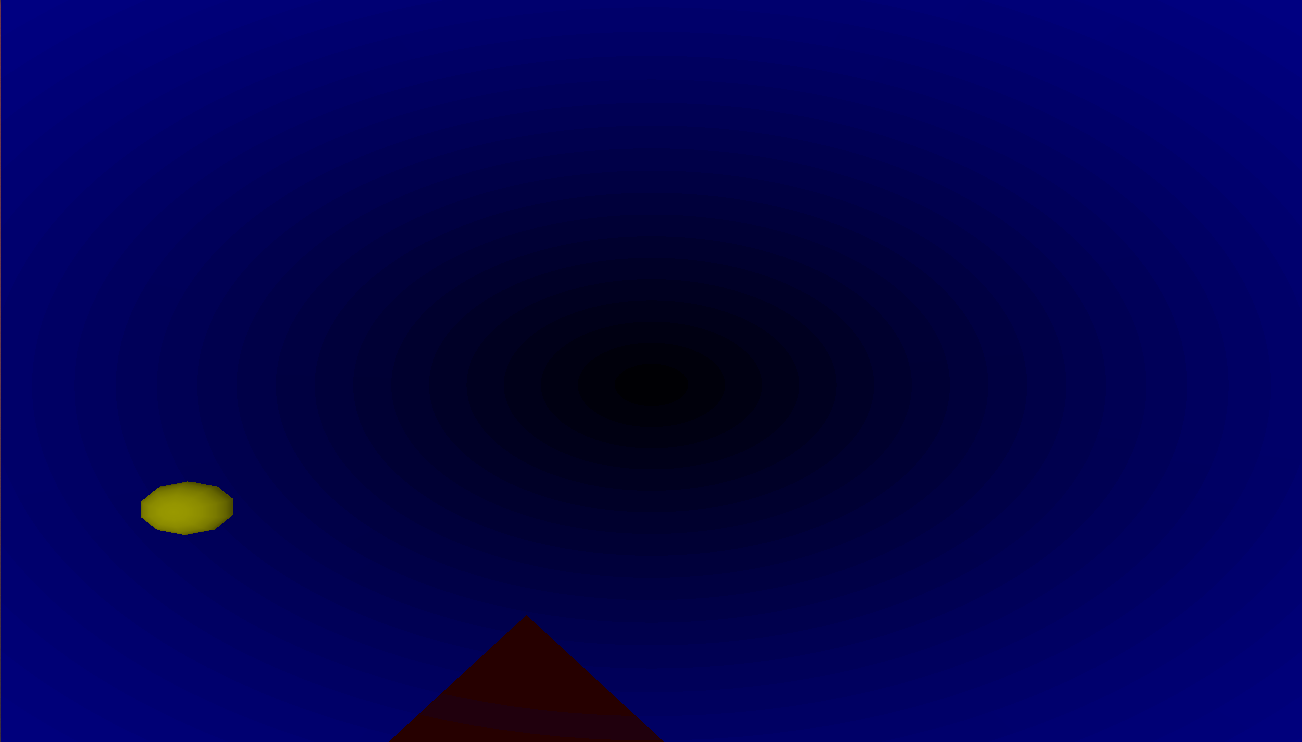
\includegraphics[width=1\linewidth]{lambert-screen.png}

Скриншот программы для зеркального отражения:


\includegraphics[width=1\linewidth]{zerkalo-screen.png}

Проекции сферы излучения (слева -- диффузное, справа -- зеркальное):


\includegraphics[width=0.499\linewidth]{lambert-map.png}
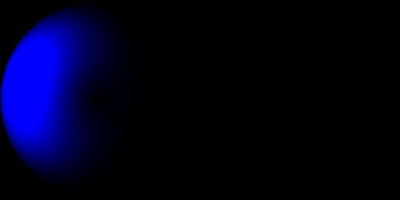
\includegraphics[width=0.499\linewidth]{zerkalo-map.png}

Таким образом, у нас есть возможность достаточно гибко моделировать различные материалы. 

\subsection*{Первичные и вторичные}

Рассмотрим одно положение объектов и сравним разницу между картинами в первом случае создаваемой только первично-освещенными областями и во втором -- совокупностью первичных и вторичных групп полигонов. 

Первично-освещенные области:

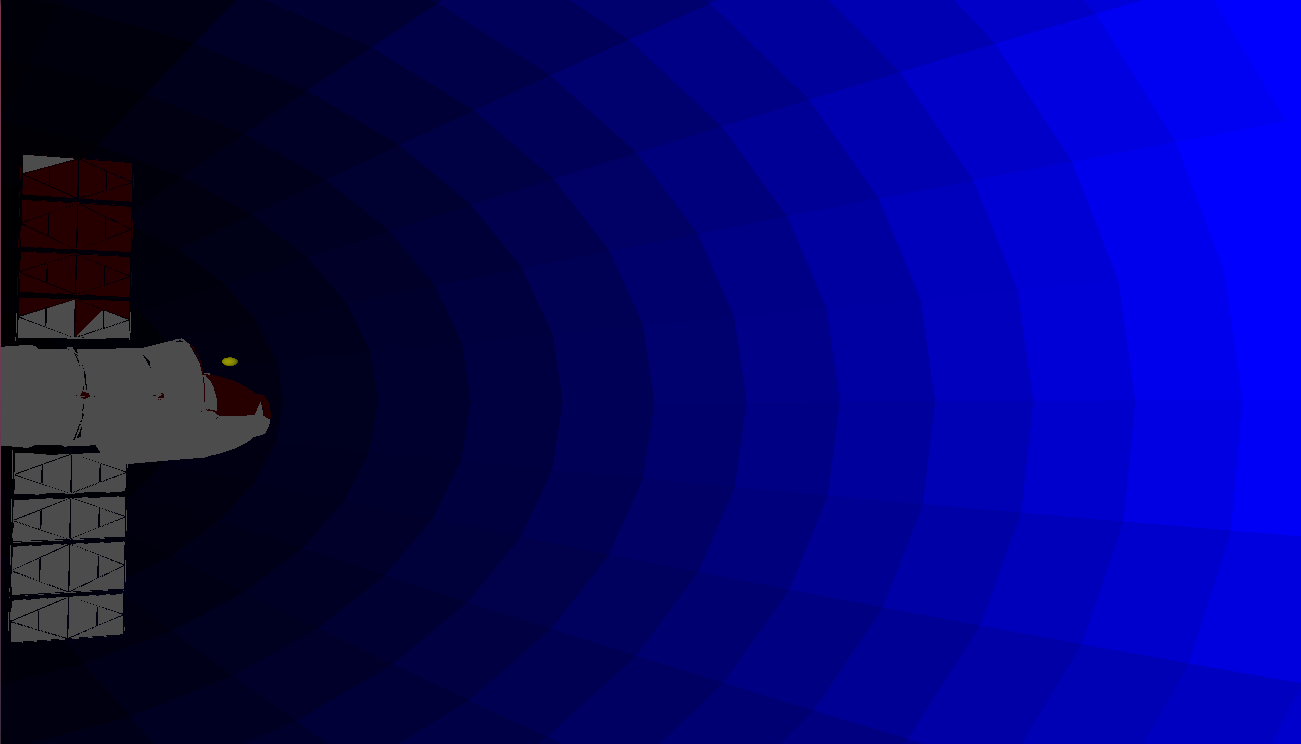
\includegraphics[width=0.499\linewidth]{first-screen-1.png}
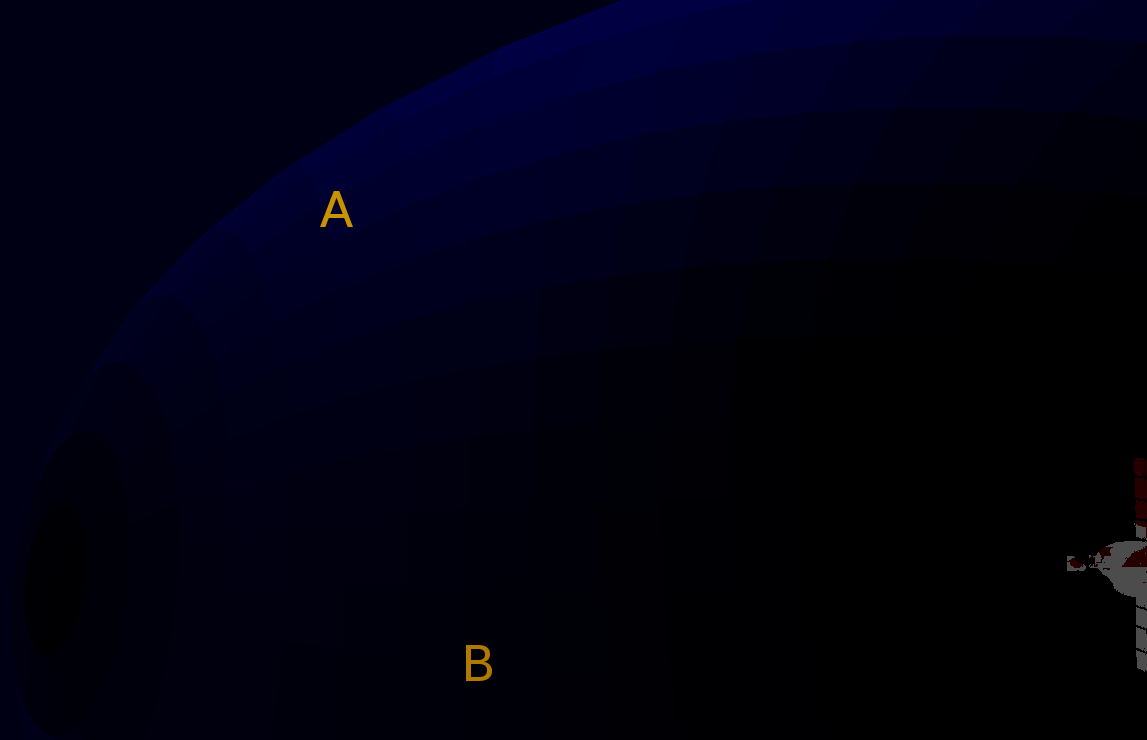
\includegraphics[width=0.499\linewidth]{first-screen-2.png}

Вторично-освещенные фрагменты:

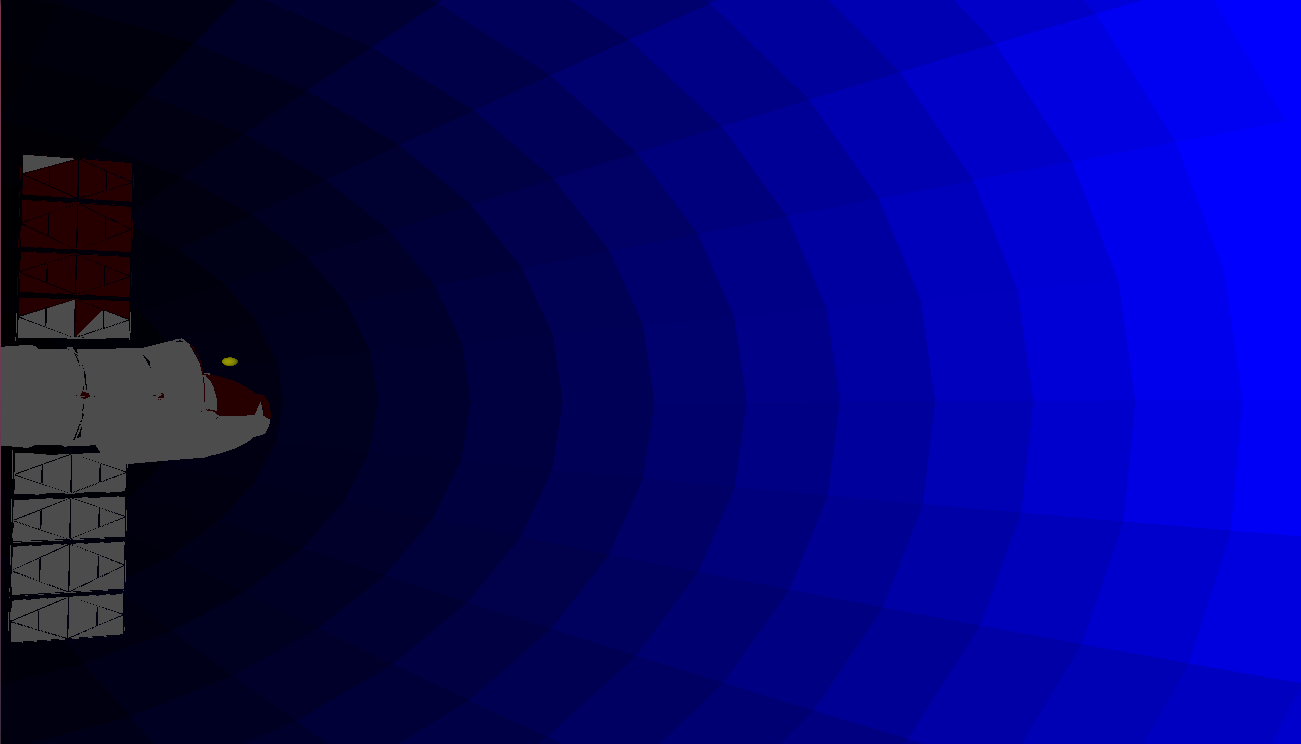
\includegraphics[width=0.499\linewidth]{first-screen-1.png}
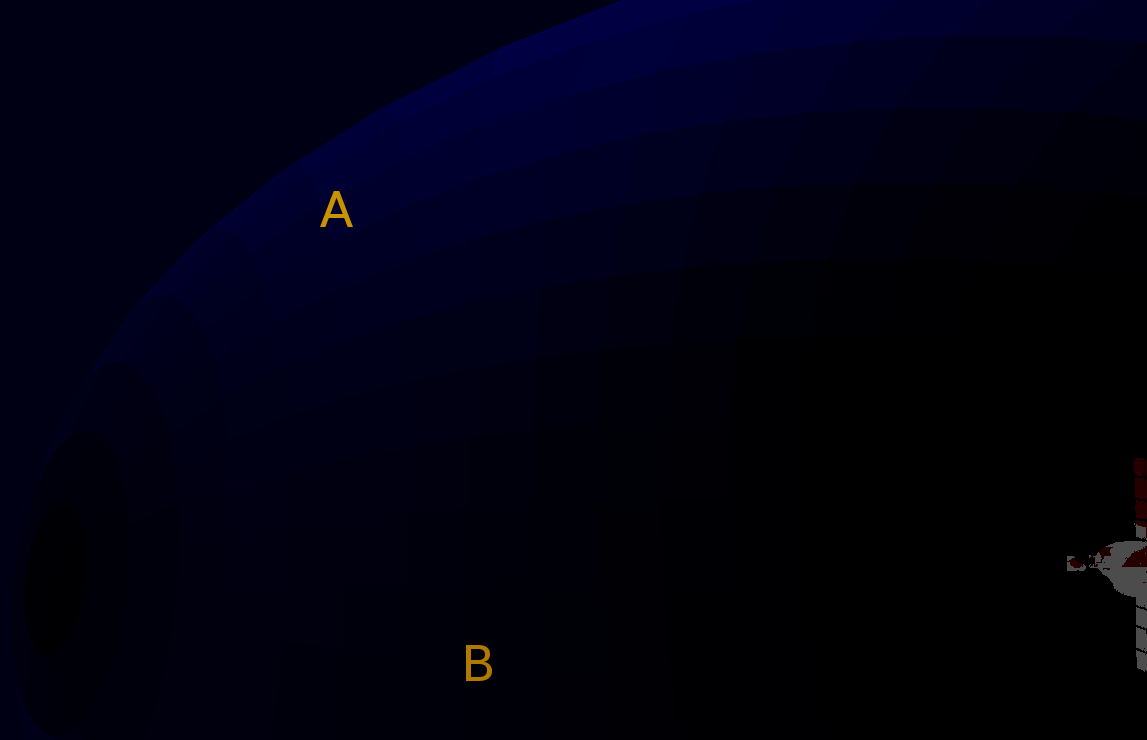
\includegraphics[width=0.499\linewidth]{first-screen-2.png}

Проекции сферы излучения (слева -- только первичные, справа первичные и вторичные области):

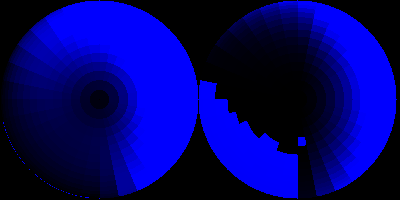
\includegraphics[width=0.499\linewidth]{first-map.png}
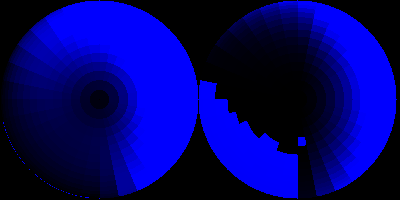
\includegraphics[width=0.499\linewidth]{first-map.png}

\subsection*{Сравнение производительности}

Проведем сравнение производительностей по моделированию поставленных нами задач. Помимо параллельной версии программы, запускаемой на графическом ускорителе, была написана последовательная версия программы, запускаемая на центральном процессоре.  

Характеристики центрального процессора (CPU): модель Intel Core 2 Duo T6600, тактовая частота 2200 MHz. 

Несмотря на то, что процессор многоядерный, программа была написана последовательно, то есть во время исполнении занято было только одно ядро.

Характеристики графического ускорителя (GPU): чипсет Nvidia GeForse GT 240M, объем 1024 mb.

Сравнение проводилось на трех сложных одинаковых полигональных моделях слонов с разной степенью детализации.

\begin{center}
\begin{tabular}{cccc}
\textbf{время в сек.}		& \textbf{слон 1148 гр} 			& \textbf{слон 10152 гр}		& \textbf{слон 39292 гр} 		\\
CPU 							& 0					 				& 0									& 0			 						\\
GPU 							& 0									& 0 									& 0									\\
ускорение 					& 0									& 0									& 0 									\\
\end{tabular}
\end{center}







